\documentclass[8pt]{beamer}
\setbeamertemplate{navigation symbols}{}

\usepackage{multicol}
\usepackage{graphicx}
\usepackage{soul}
\usepackage{tikz}
\graphicspath{ {images/} }
\usecolortheme{beaver}


\begin{document}

%Title pages
\title{Ex vs. Teco}
\author{Brandon Moore and John Markiewicz}
\date{}

\begin{frame}
  \titlepage
\end{frame}

\title{Neo-Vim vs Spacemacs}
\author{Brandon Moore and John Markiewicz}
\date{}

\begin{frame}
  \titlepage
\end{frame}
%End title pages

\title{Vim vs. Emacs}
\author{Brandon Moore and John Markiewicz}
\date{}

\begin{frame}
  \titlepage
\end{frame}

\begin{frame}
  \frametitle{C-x M-c M-butterfly}
  \begin{quote}
    Emacs is a great operating system, lacking only a decent editor
  \end{quote}
        \begin{flushright}
          --Anonymous
        \end{flushright}
\end{frame}
\note{A vim-user's view of Emacs is that the editor has a heavy amount of features, but lacks a focus on actually editing and tries to do everything under the sun.}

\begin{frame}
  \frametitle{vi vi vi}
  \begin{quote}
    Using a free version of vi is not a sin but a penance.
  \end{quote}
  \begin{flushright}
    \only<1>{--Richard Stallman, head of the Church of Emacs\\}
        \only<2>{--\st{Richard Stallman, head of the Church of Emacs}\\}
        \only<2>{--Saint IGNUcious, head of the Church of Emacs}
  \end{flushright}
\end{frame}
\note{Emacs view on Vim: it's fine to use, but why limit yourself like that?}

\begin{frame}
  \frametitle{A historic holy war\\Emacs vs. Vi(m)}
\begin{tikz}
  [
    grow                    = right,
    sibling distance        = 6em,
    level distance          = 7em,
    edge from parent/.style = {draw, -latex},
    every node/.style       = {font=\footnotesize},
    sloped
  ]
  \node{Ed(1971)}
    child {
      node{Ex(1976)}
      child {
        node{Vi(1976)}
        child {
          node{Vim(1991)}
          child {
            node{NeoVim}
          }
        }
      }
    }
    child {
      node{Teco(1962)}
      child {
        node{Emacs(1976)}
        child {
          node{GNU Emacs(1985)}
          child {
            node{Spacemacs}
          }
        }
      }
    };
\end{tikz}
\end{frame}
\note{History of the editors}

\begin{frame}
  
\includegraphics[width=.5\textwidth]{vim_logo.png}
  
\includegraphics[width=.5\textwidth]{emacs_logo.png}
\end{frame}

\begin{frame}
  \frametitle{Let's look at Vim}
  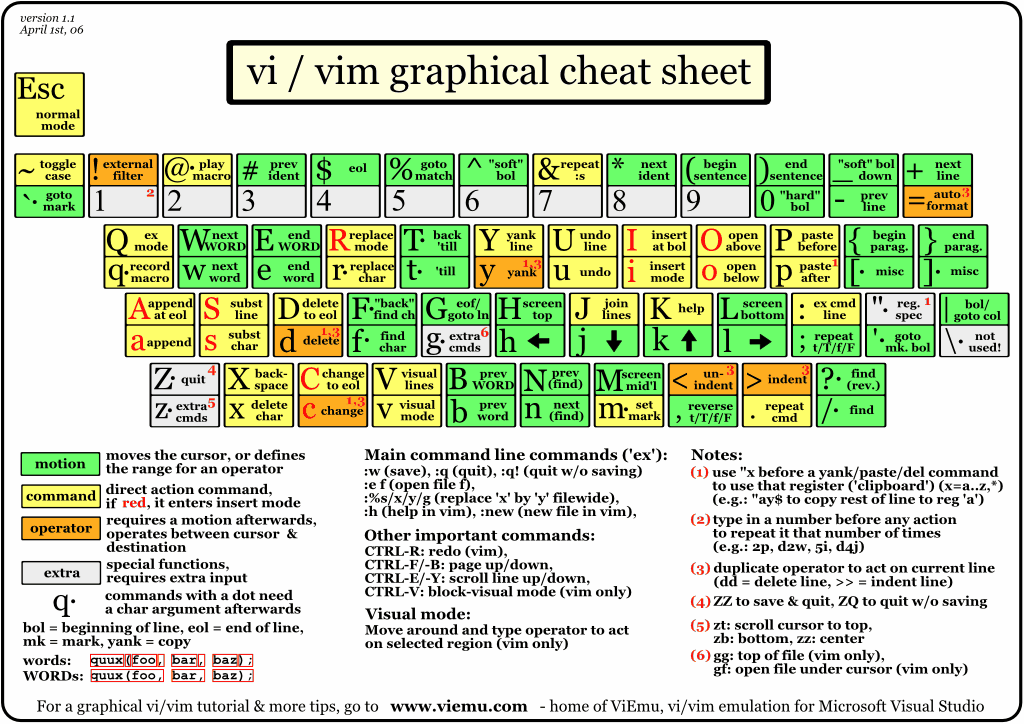
\includegraphics[width=\textwidth]{vim_cheatsheet.png}
\end{frame}
\note{Demonstrate Vim}

\begin{frame}
  \frametitle{Let's look at Emacs}
  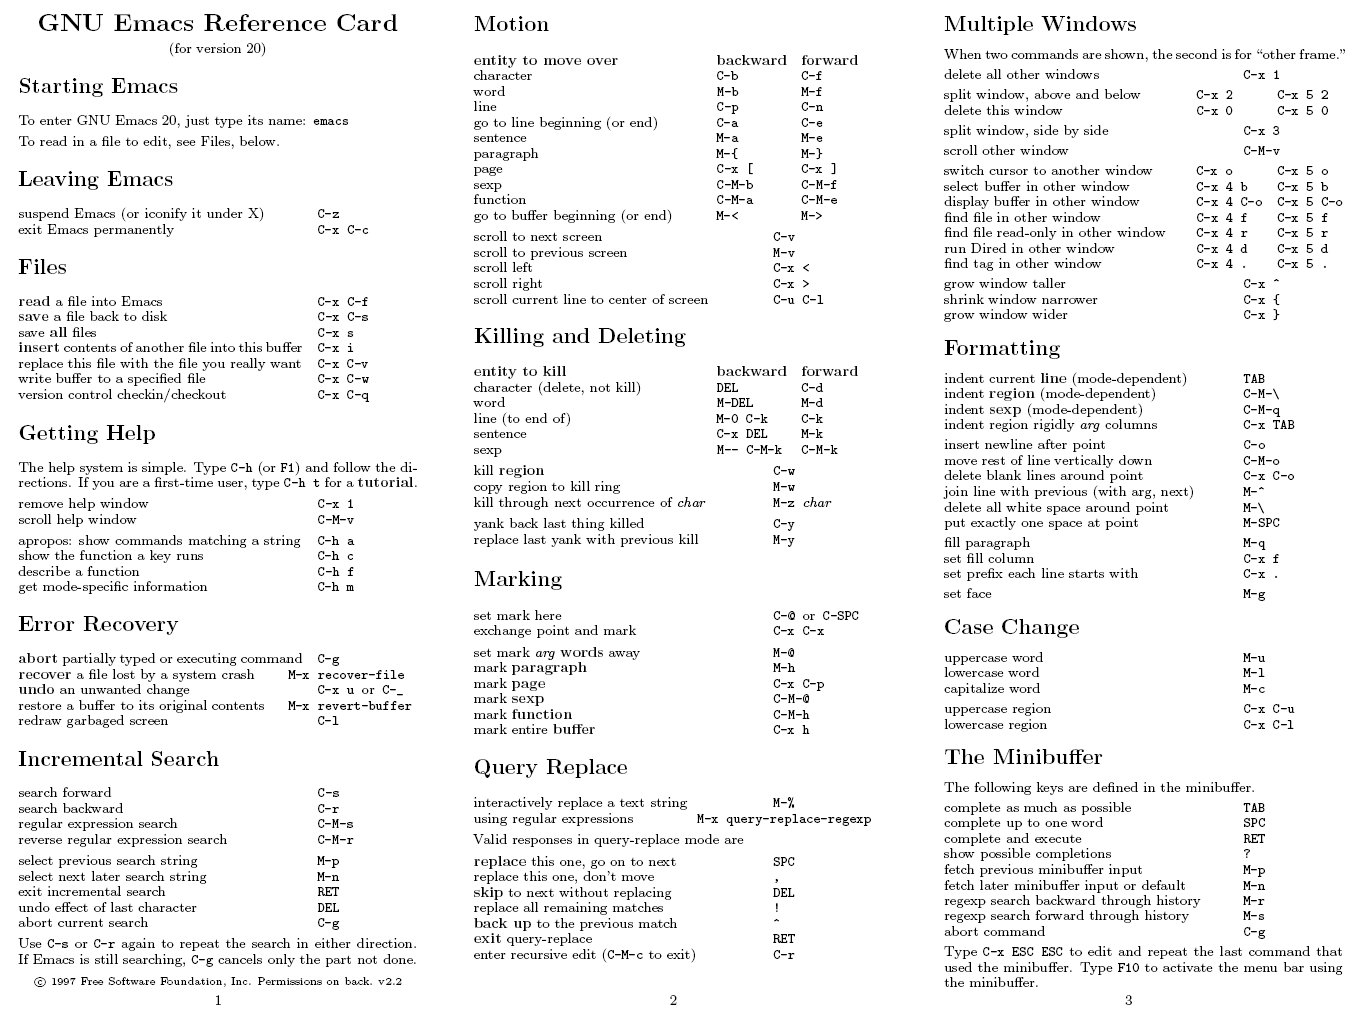
\includegraphics[width=\textwidth]{emacs_cheatsheet.jpg}
\end{frame}
\note{Demonstrate Emacs}

\begin{frame}
  \frametitle{Why use Vim?}
  \begin{multicols}{2}
    \textbf{Pros of Vim}
    \begin{itemize}
      \item Customizable
      \item Rich library of extensions
      \item Constantly improving
      \item Portable
      \item ...in multiple ways
    \end{itemize}
    \columnbreak
    \textbf{Cons of Emacs}
    \begin{itemize}
      \item Reliant on customization
      \item Comes with bloat
      \item Hello Carpal Tunnel
      \item Tries to do too much
    \end{itemize}
  \end{multicols}
\end{frame}
\note{Malide's pro con slide}

\begin{frame}
  \frametitle{Why use Emacs?}
  \begin{multicols}{2}
    \textbf{Pros of Emacs}
    \begin{itemize}
      \item Flexible, powerful, pleasant to use language for adding
        features (elisp).
      \item Features.
      \item Compatibility with the past few decades' worth of software
      \item Org-mode
      \item Evil-mode for those used to vim keybindings
    \end{itemize}
    \columnbreak
    \textbf{Cons of Vim}
    \begin{itemize}
      \item Community fragmentation (Neovim vs Vim 8.0) and
        incompatibility between versions.
      \item Fewer features.
      \item Vimscript.
      \item Inconsistent async methods between Vim 8 and Neovim.
      \item Performance issues with syntax highlighting/line
        numbers/large files.
    \end{itemize}
  \end{multicols}
\end{frame}
\note{EDT's pro con slide}

\begin{frame}
  \frametitle{stdlinux (and problems with old systems)}
        \begin{itemize}
          \item stdlinux is old and out of date. vim and emacs don't work well
          \item a basic .vimrc is needed to use vim on stdlinux
          \item It should be updated soon!
        \end{itemize}
\end{frame}

\begin{frame}
  \frametitle{How to learn}
  \textbf{Vim}
  \begin{itemize}
    \item vim help pages (via :help $<$topic$>$)
    \item \$vimtutor
    \item http://www.openvim.com/
  \end{itemize}
  \textbf{Emacs}
  \begin{itemize}
    \item Emacs help features (internal documentation accessible via C-h C-a)
    \item Emacs wiki
    \item Worg (for org-mode)
  \end{itemize}
\end{frame}
\note{List of resources}

\begin{frame}
  \Huge{https://moore3071.github.io/vim\_vs\_emacs}
\end{frame}

\end{document}
